\chapter{Background}
\label{ch:background}

\emph{In this chapter the notation, phrases and concepts that are used throughout the document are explained.}
\emph{An overview of general model alignment as well as the specifics of alignment via steering adaptors is described.}
\emph{This includes a history of the different techniques and the details of the four methods used in this project.}

\emph{The history of large language models and why they are important in current research is outline.}
\emph{Additionally the challenges that are faced in interpreting these large models is explained.}
\emph{The solutions to these challenges present possible metrics that can be used to analyse the effectiveness of steering adaptors.}

\section{Notation and Concepts}

Model ``behaviours", in general, are patterns in how the model responds to input.
This includes the desired behaviour it was trained on (such as classifying images of cats and dogs) but includes patterns in the output that were not explicitly trained for.
Desired model behaviour (such as responding truthfully) is considered ``positive" and undesired model behaviour (such as lying or subverting) is considered ``negative".
Specifically, an example of the desired behaviour is considered a ``positive example'' and an example of undesired or neutral behaviour is considered a ``negative'' example.
An example of a behaviour generally includes an input-output pairing similar to training examples (such as a picture of a cat and a response which either tells the truth, "This is a cat", or lies, "This is a dog") however they are more specific than would be using during training.
The specificity of steering examples is to insure the model adjust representations that elicit the target behaviour and avoid causing larger changes to behaviour.

When discussing NNs the concept of a ``neuron'' relates to the abstract structure that receives a real-valued, vector input and outputs a real-value scalar based on internal, learnable weights.
In practice, this is represented by a single element of a NN layer's output vector.

Vectors are represented by boldface letters, $\vx, \vy, \vz$, scalars are represented by Greek letters, $\alpha, \beta, \gamma$, and matrices are represented by boldface capital letters, $\mA, \mB, \mC$.
In general $\mR$ represents an orthonormal projection matrix into a lower dimension, $\mW$ represents a general weight matrix, and $\vb$ represents a bias vector.
Some matrices may represent transformations or collections of feature vectors, context should disambiguate the two.
In general vectors are column vectors, $\vx = \begin{bmatrix*}
    1 & 2 & \cdots & n
\end{bmatrix*}^T$ except when a collection of vectors is represented in matrix form, in this case each row is a vector.

In a multi-layer machine learning model the output of an internal layer is an ``activation'' denoted $\va$.
A positive activation is denoted $\va^+$ and a negative activation is denoted as $\va^-$. Here, ``positive activation'' means the activation extracted from the model given a positive example as above.
The mean of a set of activations, $\mathcal{A} = \{\va_i\}_{i < n}$, is denoted $\mu_\mathcal{A} = \frac{1}{n}\sum_{i=1}^{n}\va_i$.
Frequently the set of set of activations will be the positive activation or negative activation set, in this case the mean is denoted $\mu_{\va^+}$ or $\mu_{\va^-}$ respectively.

\section{Model Alignment}

As models increase in capabilities \citep{dynabench, hle, gpt-5, grok-4} they pose an increasing risk to their users \citep{c.ai, psychosis} and potentially humanity at large \citep{survellience, deepfakes, disempowerment}.
The underlying issue is that these models may be \emph{misaligned} \citep{agent-alignment}, that is to say they do not behaviour inline with users intentions.
The problem of aligning models is referred to as the \emph{alignment problem} or, within reinforcement learning \cite{rl}, the \emph{agent alignment problem} \citep{agent-alignment}.\footnote{An \emph{agent} is a reinforcement learning term for any entity that interacts with a learning environment and updates it's internal state to better achieve a predetermined goal. In this case, the model behaves as an agent.}

\citet{agent-alignment} present the agent alignment problem and propose \emph{reward modelling} as a potential avenue to align agents.
They outline a couple of assumptions as to whether reward modelling is suitable:
\begin{itemize}[nolistsep]
    \item It is possible to sufficiently learn user intentions.
    \item It is cheaper to evaluate outcomes than produce the ``correct'' behaviour.
\end{itemize}
Working on this, \citet{rlhf} apply these ideas to large language models (LLM)s.
The goal is to transform purely predictive LLMs into assistants that are ``helpful'', ``honest'', and ``harmless''.
This is achieved by utilising human feedback on LLM output as rewards for reward modelling.
The idea reinforcement learning from human feedback (RLHF) had been developed previously by \citet{rlhf-orig} but had not been applied to LLMs.
Applying the idea to modern LLMs led to the invention of the modern AI chatbot \citep{chatgpt}.

RLHF has been shown to be very effective in transforming the behaviour of models.
However, it is still possible for RLHF ``aligned'' models to be misaligned \citep{misgeneralization, c.ai}.
Furthermore, this approach to alignment is very costly requiring human annotators, reviewers and the costly process of finetuning.
Techniques to mitigate this have been proposed including RLxF \citep{alignment-survey}, utilising both human and AI feedback, representation finetuning \citep{reft}, and parameter efficient finetuning \citep{peft}.

Representation finetuning or more generally representation engineering \citep{steering-taxonomy} presents a promising avenue for alignment \citep{steering-clear, steering-theory, steering-taxonomy}.
Rather than requiring large amounts of human annotated data and changing model weights only the representations need editing.
This manipulation of representations can occur after model training, with a smaller dataset, and incurs limited overheads during inference.
This thesis focuses on \emph{steering adaptors}, a subset of representation engineering.

\section{Steering Adaptors}

The general form of a steering adaptor is a simple module that augments a layer's output.
The idea is to change the internal representation away from a harmful or misaligned concept towards one that is aligned to the users intentions.
The goal is to keep all other aspects of the representation intact so that the performance of the model is not hindered.

Rather than large amounts of annotated data or large weight matrices these techniques require a handful of positive and negative examples.
Given their lightweight nature these techniques have shown promising results \citep{steering-taxonomy, steering-theory, steering-clear, reft}.

\subsection{Contrastive Activation Addition (CAA)}
\label{caa}

An intuitive approach to model intervention is to perturb the model's activations in a desired direction.
By calculating a linear direction in activation space from undesired activations towards desired ones this vector can simply be added to all activations in the model during inference.
The hope is that the model produces output that matches the desired behaviour whilst maintaining the context of the new input.

\begin{figure}
    \centering
    \captionsetup{width=.9\textwidth}
    \begin{tikzpicture}

\foreach \i in {1,...,100} {
    % generate random coords and save them in dedicated macros
    \pgfmathsetmacro{\rr}{rnd*2}       % x in [0,6]
    \pgfmathsetmacro{\rtheta}{rnd*360}   % y in [-3,3]
    \node[red] at ({\rr*cos(\rtheta)},{\rr*sin(\rtheta)}) {$\times$};
}

% Second set (green crosses), horizontally shifted
\foreach \i in {1,...,100} {
    \pgfmathsetmacro{\rr}{rnd*2}       % x in [0,6]
    \pgfmathsetmacro{\rtheta}{rnd*360}   % y in [-3,3]
    \node[green!70!black] at ({7+\rr*cos(\rtheta)},{\rr*sin(\rtheta)}) {$\times$};
}

% Draw mean points
\node[circle, fill=red, inner sep=3pt, label={[yshift=4em,xshift=-4em]$\mu_{\va^-}$}] (meanA) at (0,0) {};
\node[circle, fill=green!70!black, inner sep=3pt, label={[yshift=4em,xshift=4em]$\mu_{\va^+}$}] (meanB) at (7,0) {};

% Draw dashed arrow between means
\draw[dashed, -{Stealth[length=3mm]}, thick] (meanA) -- (meanB)
    node[midway, above] {$\vv_{steer} = \mu_{\va^+} - \mu_{\va^-}$};

% Draw random point to steer
\node[rectangle, fill=black, inner sep=2pt] (test) at (1, 1) {};
\node[rectangle, fill=green!70!black, inner sep=2pt] (steered) at (8, 1) {};

% Draw dashed arrow between steered points
\draw[-{Stealth[length=3mm]}, thick] (test) -- (steered)
    node[midway, above] {$\va_{steer} = \va + \vv_{steered}$};

\end{tikzpicture}

    \caption{Demonstration of contrastive activation addition \citep{caa}. The figure represents a simple representation space of dimension 2 with clear separability. The average displacement between negative behaviour, $\vmu_{\va^-}$, and positive behaviour, $\vmu_{\va^+}$, represents the direction the target concept lies on. Applying this to a new point (black square) produces a new point (green square) with the desired behaviour whilst maintaining unrelated properties.}
    \label{fig:caa}
\end{figure}

In the simplest form consider two example inputs, \texttt{The prime minister of the UK is Count Binface} and \texttt{The prime minister of the UK is Sir Kier Starmer},  representing undesired (untruthful) and desired (truthful) behaviour.
The model represents these two sentences with minor differences in its internal representation space.
The difference of these representations gives a direction in feature space that corresponds to shifting the models output from undesired behaviour towards desired behaviour (a ``truthfulness'' direction).
Importantly, the context of the output is maintained, ``who is the prime minister of the UK?'', but the model no longer produces the undesired (false) string, ``Count Binface''.
This is the approach proposed by \citet{activation-addition}, however, it is not robust and relies heavily on the example inputs \citep{caa}.

To improve on this approach \citet{caa} suggest using a collection of examples and calculating their mean difference in activation space.
This requires the notion of \emph{contrastive pairs}, two inputs that are similar in all ways except for the behaviour that is being changed.
Hence, this approach is known as \emph{contrastive activation addition} (CAA).
This process is demonstrated in \cref{fig:caa}.

Formally, given a set of positive example activations $(\va_i^+)_{i\le n}$ and negative example activations $(\va_i^-)_{i\le n}$ a \emph{steering vector} for this behaviour is
\[\vv_{steer} = \frac{1}{n}\sum_{i=1}^{n}\left(\va_i^+ - \va_i^-\right).\]

Given a steering vector, $\vv_{steer}$, and a model activation during inference, $\va$, the resulting steered activation is
\begin{equation}
    \label{eq:caa}
    \va_{steered} = \va + \lambda\vv_{steer}
\end{equation}
where $\lambda$ is a user-defined parameter controlling the strength of the steering intervention.
The model activation is replaced by the steered activation during inference resulting in the model producing an output aligned with the positive examples.

This approach has a few drawbacks \citep{steerability, ace, non-linear-features} due to its assumptions.
Primarily this approach does not consider how much of a behaviour is already present.
This means the steering parameter does not fully determine the strength of the desired behaviour.
Furthermore, \citet{steerability} demonstrate that CAA is unable to consistently steer a model towards target behaviours and in some cases may steer the model \emph{towards the negative behaviour}.
The approach assumes that concepts in activation space are linear which \citet{non-linear-features} show is not universal.
Techniques such as affine concept editing (ACE) \cref{sec:ace} use an affine approach to overcome these drawbacks.

\subsection{Affine Concept Editing (ACE)}
\label{sec:ace}

\citet{ace} claim that CAA \citep{caa} is not sufficiently general as it does not consider how much the desired behaviour is already present.
To see this consider an arbitrary activation vector $\va$ and steering direction $\vr$ encoding some behaviour.
$\va$ can be decomposed as the perpendicular and parallel components of $\vr$
\begin{equation}
    \label{eq:components}
    \begin{aligned}
        \va &= \text{proj}_\vr^{\perp}(\va) + \text{proj}_\vr^{\parallel}(\va) \\
            &= \text{proj}_\vr^{\perp}(\va) + \alpha\vr.
    \end{aligned}
\end{equation}
This shows that CAA \citep{caa} does not account for how much a behaviour may already be present in an activation, represented by $\alpha\vr$.
However $\alpha = 0$ is not necessarily the absence of the target behaviour, that is, it is not (generally) the case that $\mathbf{0}$ represents lack of behaviour.
Instead assume some vector $\va_0$ represents the lack of the target behaviour.
\cref{eq:components} can incorporate this idea as follows
\begin{align*}
    \va &= \va_0 + \Delta\va \\
        &= \va_0 + \text{proj}_\vr^{\perp}(\Delta\va) + \text{proj}_\vr^{\parallel}(\Delta\va) \\
        &= \va_0 + \text{proj}_\vr^{\perp}(\Delta\va) + \alpha^\prime\vr.
\end{align*}

Removing the behaviour by setting $\alpha^\prime = 0$ yields
\begin{align*}
    \va^\prime &= \va_0 + \text{proj}_\vr^{\perp}(\Delta\va) \\
               &= \va - \text{proj}_\vr^{\parallel}(\Delta\va) \\
               &= \va - \text{proj}_\vr^{\parallel}(\va) + \text{proj}_\vr^{\parallel}(\va_0) \\
               &= \va - \text{proj}_\vr^{\parallel}(\va) + \alpha_0\vr.\footnotemark[1]
\end{align*}

\begin{figure}
    \centering
    \captionsetup{width=.9\textwidth}
    \begin{tikzpicture}
% DRAW CAA
% Draw dashed axes
\node[] (bstart) at (-1, -1) {};
\node[] (bend) at (3, 3) {};
\node[] (pstart) at (1, -1) {};
\node[] (pend) at (-3, 3) {};

\draw[dashed, thick] (bstart) -- (bend);
\draw[dashed, thick] (pstart) -- (pend);

% Draw origin
\node[circle, fill=black, inner sep=2pt, label={$O$}] (originA) at (0, 0) {};

% Draw means
\node[circle, fill=black, inner sep=2pt, label={[xshift=1.5em, yshift=-1em]$\mu_{\va^-}$}] (meanA) at (0.5, 1.5) {};
\node[circle, fill=black, inner sep=2pt, label={$\mu_{\va^+}$}] (meanB) at (-0.5, 2.5) {};

% Draw arrow between means
\draw[dashed, -{Stealth[length=3mm]}, thick] (meanA) -- (meanB)
    node[midway, right] {$\vv_{steer}$};

% Draw 'random' points and steer
\node[draw, circle, red, dashed, inner sep=2pt] (test1A) at (-0.7, 1.7) {};
\node[circle, fill=green!70!black, dashed, inner sep=2pt] (test1B) at (-1.7, 2.7) {};

\node[draw, circle, red, dashed, inner sep=2pt] (test2A) at (1, 2.5) {};
\node[circle, fill=green!70!black, dashed, inner sep=2pt] (test2B) at (0, 3.5) {};

\draw[blue!70, -{Stealth[length=3mm]}, thick] (test1A) -- (test1B);
\draw[blue!70, -{Stealth[length=3mm]}, thick] (test2A) -- (test2B);

\node[draw, fit=(bstart) (bend) (pstart) (pend) (test2B), label={CAA}] {};


% DRAW ACE
% Draw dashed axes
\node[] (bstart) at (6, -1) {};
\node[] (bend) at (10, 3) {};
\node[] (pstart) at (8, -1) {};
\node[] (pend) at (4, 3) {};

\draw[dashed, thick] (bstart) -- (bend);
\draw[dashed, thick] (pstart) -- (pend);

% Draw origin
\node[circle, fill=black, inner sep=2pt, label={$O$}] (originA) at (7, 0) {};

% Draw means
\node[circle, fill=black, inner sep=2pt, label={[xshift=1.5em, yshift=-1em]$\mu_{\va^-}$}] (meanA) at (7.5, 1.5) {};
\node[circle, fill=black, inner sep=2pt, label={$\mu_{\va^+}$}] (meanB) at (6.5, 2.5) {};

% Draw arrow between means
\draw[dashed, -{Stealth[length=3mm]}, thick] (meanA) -- (meanB)
    node[midway, right] {$\vv_{steer}$};

% Draw 'random' points and steer
\node[draw, circle, red, dashed, inner sep=2pt] (test1A) at (6.3, 1.7) {};
\node[circle, fill=green!70!black, dashed, inner sep=2pt] (test1B) at (6, 2) {};

\node[draw, circle, red, dashed, inner sep=2pt] (test2A) at (8, 2.5) {};
\node[circle, fill=green!70!black, dashed, inner sep=2pt] (test2B) at (7.25, 3.25) {};

\node[] (upper) at (7, 3.48) {};

\draw[blue!70, -{Stealth[length=3mm]}, thick] (test1A) -- (test1B);
\draw[blue!70, -{Stealth[length=3mm]}, thick] (test2A) -- (test2B);

\node[draw, fit=(bstart) (bend) (pstart) (pend) (upper), label={ACE}] {};

\node[draw, fit=(bstart) (bend) (pstart) (pend) (upper), label={ACE}] {};

\end{tikzpicture}

    \caption{A comparison of CAA \citep{caa} and affine concept editing \citep{ace}. This is a reproduction of Figure 1 in \citet{ace} with the steering towards the positive examples instead. Compared to CAA, ACE does not adjust perpendicular components but correctly adjusts those parallel to the steering direction.}
    \label{fig:ace}
\end{figure}

This represents the activation lacking the target behaviour but retaining other relevant context.
\footnotetext[1]{As $\va_0$ exists as a reference point along the steered direction.}
The behaviour can be reintroduced at any relevant strength resulting in
\begin{equation}
    \label{eq:ace}
    \va_\text{steered} = \va_0 - \text{proj}_\vr^{\parallel}(\va) + \alpha_0\vr + \alpha\vr.
\end{equation}

This process is described graphically in \cref{fig:ace}.

Given positive example activations $(\va_i^+)_{i\le n}$ and negative example activations $(\va_i^-)_{i\le n}$ the reference point and steering direction are
\begin{align*}
    \vr = \frac{1}{n}\sum_{i=1}^{n}(\va_i^+ - \va_i^-) && \alpha_0 = \text{proj}_\vr^\parallel\left(\frac{1}{n}\sum_{i=1}^{n}\va_i^-\right)
\end{align*}
A proof that these definitions are the optimal assignments is presented in \cref{app:ace}.

This approach is no longer a linear edit to the activations and now includes a bias term, $\va_0$.
This is therefore affine and hence the name \emph{affine concept editing}.

\subsection{Low-rank Representation Finetuning (LoReFT)}
\label{loreft}

Both CAA \citep{caa} and ACE \citep{ace} edit the activations in their full rank form and rely on addition (whether affine or linear).
This limits the transforms the approaches can apply to the activation space.
If the desired behaviour requires rotations or scaling of the activations these methods fail.
However, perform affine transformations to the full rank activation is costly as the dimension of the activations may be large.

\citet{reft} present a low-rank steering adaptor inspired by parameter-efficient finetuning methods such as LoRA \citep{lora}, DoRA \citep{dora} and adaptor-based methods \citep{petl}.
Unlike steering these approaches aim to finetune a model using reduced parameter counts compared to the original model.
This approach uses a small set of parameters that augment a model layers output, these can be trained whilst the original model weights remain the same greatly reducing the number of parameters needed to be trained.

Rather than finetuning a model, LoReFT edits the representations of the model, equivalent to steering.
To reduce the parameter count this learnable steering is performed in a low-rank space.
The specific approach is based on the distributed interchange intervention \citep[DII]{dii}.
DII is a version of interchange intervention whereby a causal model (with human understandable structure) is aligned with a neural network (NN) that exhibits the same behaviour.
By identifying possible neurons that exhibit the same behaviour as intermediate nodes in the causal model it is possible to intervene with the neuron's value across different inputs and verify the output behaviour matches how the causal model behaves.
This is a very similar to that of steering adaptors except there is no associated causal model, simply an alignment goal.
Rather than brute-force search for a causal node's corresponding neuron, \citet{dii} suggest projecting the respresentations into a lower dimensional space, comparing the causal node value and the NNs neuron, then projecting back.
\citet{reft} present the following form of DII for the case of representation finetuning.
\begin{equation*}
    DII(\vx,\vy,\mR) = \vx + \mR^T(\mR\vy - \mR\vx)
\end{equation*}
where $\mR \in \mathbb{R}^{r\times d}$ is a low-rank projection matrix.

\begin{figure}
    \centering
    \captionsetup{width=.9\textwidth}
    \begin{tikzpicture}[node distance=0.3cm]
    % Draw LLM
    % Draw nodes
    \node[
        draw,
        fill=black!30,
        minimum width=2cm,
        inner ysep=0.2cm,
        rounded corners
    ] (layer1) at (0, 0) {};
    \node[
        draw,
        fill=black!30,
        minimum width=2cm,
        inner ysep=0.2cm,
        rounded corners,
        above = of layer1
    ] (layer2) {};
    \node[
        draw,
        fill=black!30,
        minimum width=2cm,
        inner ysep=0.2cm,
        rounded corners,
        above = of layer2
    ] (layer3) {};
    \node[
        draw,
        fill=black!30,
        minimum width=2cm,
        inner ysep=0.2cm,
        rounded corners,
        above = of layer3
    ] (layer4) {};
    \node[
        draw,
        fill=black!30,
        minimum width=2cm,
        inner ysep=0.2cm,
        rounded corners,
        above = of layer4
    ] (layer5) {};
    \node[
        draw,
        fill=black!30,
        minimum width=2cm,
        inner ysep=0.2cm,
        rounded corners,
        above = of layer5
    ] (layer6) {};

    \node[right = 0.1cm of layer4] (outer) {};

    % Connect them up
    \draw[thick, ->, >=stealth] ($(layer1) + (0,-0.75)$) -- (layer1.south);
    \draw[thick, ->, >=stealth] (layer1.north) -- (layer2.south);
    \draw[thick, ->, >=stealth] (layer2.north) -- (layer3.south);
    \draw[thick, ->, >=stealth] (layer3.north) -- (layer4.south);
    \draw[thick, ->, >=stealth] (layer4.north) -- (layer5.south);
    \draw[thick, ->, >=stealth] (layer5.north) -- (layer6.south);
    \draw[thick, ->, >=stealth] (layer6.north) -- ++(0,0.5);

    % Draw Adaptor
    % Draw nodes
    \node[
        draw,
        fill=green!70,
        minimum width=1cm,
        rounded corners,
        inner ysep=0.2cm,
        left = 1.5cm of layer4
    ] (base) {};
    \node[
        draw,
        fill=white,
        left = -0.4cm of base
    ] (bit1) {};
    \node[
        draw,
        fill=black!50,
        right = 0.01cm of bit1
    ] (bit2) {};
    \node[
        draw,
        fill=white,
        right = 0.01cm of bit2
    ] (bit3) {};
    \node[
        draw,
        fill=green!70,
        trapezium,
        trapezium angle=60,
        minimum width=1.5cm,
        below = 0.25cm of base
    ] (R) {R};
    \node[
        draw,
        minimum width=1.5cm,
        rounded corners,
        inner ysep=0.2cm,
        below = of R,
    ] (input) {};
    \node[
        draw,
        fill=black!50,
        left = -0.35cm of input
    ] (bit1) {};
    \node[
        draw,
        right = 0.01cm of bit1
    ] (bit2) {};
    \node[
        draw,
        fill=black!25,
        right = 0.01cm of bit2
    ] (bit3) {};
    \node[
        draw,
        fill=black!90,
        right = 0.01cm of bit3
    ] (bit4) {};
    \node[
        draw,
        fill=black!10,
        right = 0.01cm of bit4
    ] (bit5) {};
    \node[
        draw,
        fill=yellow!70,
        minimum width=1cm,
        rounded corners,
        inner ysep=0.2cm,
        left = 2cm of base
    ] (source) {};
    \node[
        draw,
        fill=black!70,
        left = -0.4cm of source
    ] (bit1) {};
    \node[
        draw,
        fill=black!20,
        right = 0.01cm of bit1
    ] (bit2) {};
    \node[
        draw,
        fill=white,
        right = 0.01cm of bit2
    ] (bit3) {};
    \node[
        draw,
        fill=yellow!70,
        trapezium,
        trapezium angle=60,
        minimum width=1.5cm,
        below = 0.25cm of source
    ] (W) {W};
    \node[
        draw,
        minimum width=1.5cm,
        rounded corners,
        inner ysep=0.2cm,
        left = 1.5cm of input,
    ] (input2) {};
    \node[
        draw,
        fill=black!50,
        left = -0.35cm of input2
    ] (bit1) {};
    \node[
        draw,
        right = 0.01cm of bit1
    ] (bit2) {};
    \node[
        draw,
        fill=black!25,
        right = 0.01cm of bit2
    ] (bit3) {};
    \node[
        draw,
        fill=black!90,
        right = 0.01cm of bit3
    ] (bit4) {};
    \node[
        draw,
        fill=black!10,
        right = 0.01cm of bit4
    ] (bit5) {};
    \node[
        draw,
        fill=red!30!blue!20!white,
        minimum width=1cm,
        rounded corners,
        inner ysep=0.2cm,
        label={[yshift=-0.9cm]bias},
        left = 0.5cm of base
    ] (bias) {};
    \node[
        draw,
        fill=white,
        left = -0.4cm of bias
    ] (bit1) {};
    \node[
        draw,
        fill=black!90,
        right = 0.01cm of bit1
    ] (bit2) {};
    \node[
        draw,
        fill=black!10,
        right = 0.01cm of bit2
    ] (bit3) {};
    \node[
        draw,
        fill=green!70,
        trapezium,
        trapezium angle=120,
        minimum width=1.5cm,
        above = 0.4cm of bias
    ] (RT) {$R^T$};
    \node[
        draw,
        minimum width=1.5cm,
        rounded corners,
        inner ysep=0.2cm,
        above = of RT
    ] (activation) {};
    \node[
        draw,
        left = -0.35cm of activation
    ] (bit1) {};
    \node[
        draw,
        fill=black!50,
        right = 0.01cm of bit1
    ] (bit2) {};
    \node[
        draw,
        fill=black!50,
        right = 0.01cm of bit2
    ] (bit3) {};
    \node[
        draw,
        fill=black!80,
        right = 0.01cm of bit3
    ] (bit4) {};
    \node[
        draw,
        fill=black!10,
        right = 0.01cm of bit4
    ] (bit5) {};

    % arithmetic symbols
    \node[
        left = -0.01cm of bias
    ] {$+$};
    \node[
        right = -0.01cm of bias
    ] {$-$};

    % Connect them up
    \draw[thick, ->, >=stealth] (input.north) -- (R.south);
    \draw[thick, ->, >=stealth] (input2.north) -- (W.south);
    \draw[thick, ->, >=stealth] (R.north) -- (base.south);
    \draw[thick, ->, >=stealth] (W.north) -- (source.south);
    \draw[thick, ->, >=stealth] (RT.north) -- (activation.south);

    \draw[thick, ->, >=stealth]
        (base.north)
        -- ++(0,0.2)
        -- ($(RT.south) - (0,0.2)$)
        -- (RT.south);
    \draw[thick, ->, >=stealth]
        (source.north)
        -- ++(0,0.2)
        -- ($(RT.south) - (0,0.2)$)
        -- (RT.south);
    \draw[thick, ->, >=stealth]
        (bias.north)
        -- ++(0,0.2)
        -- ($(RT.south) - (0,0.2)$)
        -- (RT.south);

    % Join the two
    \draw[thick, ->, >=stealth]
        ($(layer3.north) !0.4! (layer4.south)$)
        -- ++(-1.5,0)
        -- ($(input.south east) + (0.75,-0.3)$)
        -- ($(input.south) + (0,-0.3)$)
        -- (input.south);
    \draw[thick, ->, >=stealth]
        ($(input.south) + (0,-0.3)$)
        -- ($(input2.south) + (0,-0.3)$)
        -- (input2.south);
    \draw[thick, ->, >=stealth]
        (activation.north)
        -- ++(0,0.3)
        -- ($(activation.north east) + (2.275,0.3)$)
        -- ($(layer4.north) !0.4! (layer5.south) + (-1.5,0)$)
        -- ($(layer4.north) !0.4! (layer5.south)$);

    \node[
        draw,
        fit=(input) (input2) (activation),
        dashed,
        label={[yshift=0.3cm]Low Rank Adaptor},
        rounded corners
    ] {};
    \node[
        draw,
        fit=(layer1) (layer6),
        dashed,
        label={[yshift=0.65cm]Model},
        rounded corners
    ] {};

\end{tikzpicture}

    \caption{This figure demonstrates how the low-rank representation finetuning adaptor \citep{reft} operates. Unlike methods such as LoRA \citep{lora} this does replace the layer weights but simply adds the layer output. LoReST \citep{steering-clear} behaves similarly though the adaptor has a different architecture. This is a reproduction of Figure 2(2) in \citet{reft}.}
     \label{fig:loreft}
\end{figure}

\citet{reft} then suggest replacing $\mR\vy$ with an affine transformation $\mW\vx + \vb$.
Thus, the adaptor learns a transformation, $\mR\va^+ = \mW\va^- + \vb$, from negative activations to positive low-rank representations.
In this way the adaptor can learn low-rank representations of activations that encapsulate the desired behaviour and adjust the activations in a parameter efficient space.
The approach is therefore a \emph{low-rank representation finetuning} (LoReFT) adaptor.
The full adaptor is
\begin{equation}
    \label{eq:loreft}
    \va_\text{steered} = \va + \mR^T(\mW\va + \vb - \mR\va).
\end{equation}
The learnable parameters of the adaptor are $\phi = \{\mW, \mR, \vb\}$.
$\mR$ is constrained to be an orthogonal projection matrix achieved by differentiable QR decomposition.

Given a dataset of contrastive pairs $\mathcal{D} = (\va_i^-, \va_i^+)_{i\le n}$ the adaptor parameters $\phi$ are trained.
The goal is to accurately predict $\va_i^+$ given $\va_i^-$ as input.

Unlike CAA and ACE, LoReFT requires paired datapoints as the adaptor needs to learn a transformation from negative examples to positive examples.
This drawback means that in the low data regime this approach is less effective than the other two approaches.
However, with sufficient data, this method is able to outperform CAA and ACE as it can utilise more complex transformations between negative and positive behaviour.
The poor performance in low data regimes is improved on by \citet{steering-clear} with their low-rank representation steering adaptor.

\subsubsection{QR decomposition}

Any real-valued square matrix, $\mA$, can be decomposed as
\begin{equation*}
    \mA = \mQ\widehat\mR
\end{equation*}
where $\mQ$ is an orthogonal matrix (that is $\mQ^T = \mQ^{-1}$) and $\widehat\mR$ is upper triangular (not to be confused with $\mR$ the projection matrix above).
$\mQ$ can be viewed as a new basis where the first column of $\mA$ is normalised, then the perpendicular component of the next column of $\mA$ is normalised.
This process repeats forming a new orthonormal basis based on $\mA$.

The process described above is known as the \emph{Gram-Schmidt process}.
By running this process on a hidden matrix $\mA \in \mathbb{R}^{d\times r}$ an orthonormal matrix $\mQ \in \mathbb{R}^{d\times r}$ can be generated.
$\mQ$ can then be used as the projection matrix discussed above.

\subsection{Low-rank Representation Steering (LoReST)}
\label{lorest}

\citet{steering-clear} suggest modifying LoReFT to dynamically drop low-rank dimensions and bring the learnable bias term outside of the low-rank space.
This allows the model to perform well in the low data regime by relying on linear methods similar to CAA but keep the benefits of LoReFT.
By dynamically dropping dimensions the adaptor has more freedom to optimise the rank of the projection.

\citet{steering-clear} define an orthogonal projection
\begin{align*}
    \mP = \mI - \mR\text{diag}(\vp)\mR^T && \vp_i = \text{GumbelSoftmax}([\vl_i,0];\tau)
\end{align*}
where $\mR \in \mathbb{R}^{r\times d}$ is a learnable low-rank projection matrix, $\vl$ is a learnable Gumbel Softmax distribution probabilities, and $\tau$ is the temperature.
As with LoReFT, $\mR$ is an orthogonal projection achieved by differentiable QR decomposition.
In comparison to LoReFT \cref{eq:loreft} there is no representation editing in the low-rank space.
Instead the projection acts as a method to ``zero'' the activation similar to ACE \citep{ace}.

The full adaptor is
\begin{equation}
    \va_\text{steered} = \va - (\va\mQ)\text{diag}(\vp)\mQ^T + \vb.
\end{equation}
This approach also requires paired data to train the parameters, $\phi = \{\mQ, \vl, \vb\}$.
$\mQ$ is constrained to be orthogonal through differentiable QR decomposition.

Given a dataset of contrastive pairs $\mathcal{D} = (\va_i^-, \va_i^+)_{i\le n}$ the adaptor parameters $\phi$ are trained.
The goal is to accurately predict $\va_i^+$ given $\va_i^-$ as input.

In the low data regime the adaptor can learn to drop more dimensions and rely on $\vb$ similar to CAA \citep{caa} and ACE \citep{ace}.
As more data is available the adaptor can rely more on the low-rank projection similar to LoReFT \citep{reft}.
In this way the adaptor is able to perform consistently across different data regimes.

\subsubsection{Gumbel-Softmax}

The aim of Gumbel-Softmax is to sample from a categorical distribution whilst maintaining backpropagation.
This is useful in LoReST as it allows the adaptive selection of low-rank dimensions by modelling the choice to keep or drop a dimension as a 2 value categorical distribution.

Consider sampling from a categorical distribution with $K$ categories.
Let $X$ represent the random variable, then
\begin{equation*}
    X = \max\left\{i : \pi_1 + \pi_2 + \dots + \pi_{i-1} \le U\right\}
\end{equation*}
where $\pi_j$ is the probability of category $j$ and $U \sim Uniform(0,1)$.

Due to the $\max$ operation this is not differentiable.
Using the reparameterisation trick, and taking samples $G_i \sim Gumbel(0,1)$, $X$ can be represented as
\begin{equation*}
    \arg\max_i\left\{G_i + \log(\pi_i)\right\}.
\end{equation*}

This is still not differentiable however, when taking onehot vector representations, $\arg\max$ can be approximated by softmax.
In practice an additional temperature variable $\tau$ is introduced giving
\begin{equation*}
    x_i = \frac{\exp\left(\frac{G_i + \log(\pi_i)}{\tau}\right)}{\sum_{j}\exp\left(\frac{G_j + \log(\pi_j)}{\tau}\right)}.
\end{equation*}

As $\tau \to 0$ the computation approaches $\arg\max$ and as $\tau \to \infty$ the computation approaches uniform.

\section{Large Language Models}

Steering and model alignment in general is not confined to large language models (LLM)s however these are currently the most widespread model in use.
LLMs are trained to generate text mimicking the natural language training distribution and are characterised by incredibly large parameter counts.
Some models are as large as 671 billion \citep{deepseek} and even small models have as many as 1 billion \citep{gemma}.

LLMs are not trained to classify or fit a dataset in the classical sense but instead to produce more data as if it were sampled from the underlying training distribution.
In practice this means producing coherent natural language which they incredibly well \citep{c.ai}. The key improvement in modern LLM performance is due to the Transformer \citep{transformers} and their many derivatives \citep{linear-attention, bigbird, linformer}.

\subsection{Transformers}

Transformers \citep{transformers} are now a mainstay of modern deep learning.\footnote{This section does not aim to describe transformers in full detail but provide a sufficient background for the rest of the project.
Keywords are provided for further reading and the explanation is based on the paper by \citet{turner2023}.}
They utilise the attention mechanism to dynamically transform (sequential) input based on the surrounding context.

Attention can be considered as a learnable lookup table with queries, keys and values.
If a query and a key are similar then the corresponding value should be returned.
This can be represented as a dot-product between a matrix of queries $\mQ$ and keys $\mK$.
These are normalised to act as probabilities that a specific value is the target value.
Given a matrix of values $\mV$ attention is represented by the following equation
\begin{equation*}
    \text{softmax}\left(\frac{\mQ\mK^T}{\sqrt{d_k}}\right)\mV.
\end{equation*}
The trick is to have $\mQ$, $\mK$ and $\mV$ all depend on the input features, this is known as ``self-attention''.
In this way $\mV$ behaves like a standard weight transformation and the softmax of $\mQ$ and $\mK$ behave like a dynamic weight transformation dependent on the input.
This allows a model to ``attend" to different parts of the input by adjusting the transformation matrices that make $\mQ, \mK$ and $\mV$.

\begin{figure}
    \centering
    \captionsetup{width=.9\textwidth}
    \begin{tikzpicture}[node distance=0.5cm]
    % Draw nodes
    \node[draw, fill=red!50, minimum width=3cm, rounded corners] (embedding) at (0, 0) {Embedding};
    \node[draw, circle, above = of embedding] (pos) {};
    \node[right = 2cm of pos] (postext) {Positional Encoding};
    \node[draw, fill=orange, minimum width=3cm, rounded corners, above = of pos, align=center] (mha) {Multi-head\\Attention};
    \node[draw, fill=yellow!70, minimum width=3cm, rounded corners, above = of mha] (layernorm) {Layer Norm.};
    \node[draw, fill=blue!40, minimum width=3cm, rounded corners, above = of layernorm] (mlp) {MLP};
    \node[draw, fill=yellow!70, minimum width=3cm, rounded corners, above = of mlp] (out) {Layer Norm.};

    \node[right = 0.1cm of layernorm] (outer) {};

    % Connect them up
    \draw[thick, ->, >=stealth] ($(embedding) + (0,-0.75)$) -- (embedding);

    \draw[thick, ->, >=stealth] (embedding) -- (pos);
    \draw[thick, ->, >=stealth] (postext) -- (pos);

    \draw[thick, ->, >=stealth] (pos.north) -- ($ (pos.north) !.5! (mha.south) $) -- ++(0.75,0) -- ($ (mha.south) !.5! (mha.south east) $);
    \draw[thick, ->, >=stealth] (pos.north) -- ($ (pos.north) !.5! (mha.south) $) -- ++(-0.75,0) -- ($ (mha.south) !.5! (mha.south west) $);
    \draw[thick, ->, >=stealth] (pos.north) -- (mha.south);

    \draw[thick, ->, >=stealth] ($ (pos.north) !.25! (mha.south) $) -- ++(1.75,0) -- ($(layernorm.east) + (0.25,0)$) -- (layernorm.east);

    \draw[thick, ->, >=stealth] (mha) -- (layernorm);
    \draw[thick, ->, >=stealth] (layernorm) -- (mlp);

    \draw[thick, ->, >=stealth] ($ (layernorm.north) !.5! (mlp.south) $) -- ++(1.75,0) -- ($(out.east) + (0.25,0)$) -- (out.east);

    \draw[thick, ->, >=stealth] (mlp) -- (out);

    \draw[thick, ->, >=stealth] (out) -- ++(0,0.75);

    \node[draw, fit=(embedding) (out) (outer), dashed, rounded corners] {};
\end{tikzpicture}

    \caption{A diagram of the standard transformer decoder block. This is based on Figure 1 of \citet{transformers}. This is a single layer in a large language model where the output of one block is fed into the input of the next.}
    \label{fig:transformer}
\end{figure}

Modern Transformers contain attention blocks each containing multiple ``attention heads'' that use the above mechanism.
This allows the model to respond dynamically to a large range of inputs.
After this attention block a standard multi-layer perceptron (MLP) is added.
This constitutes the transformer block and is visualised in \cref{fig:transformer}.

The ability for Transformers to utilise context in surrounding input values makes them particularly suited to natural language processing (NLP).
The meaning of words in a sentence depend on the words that surround it.
Furthermore, the words depend on each other in different ways depending on the context.
This is precisely how transformer attention blocks work allowing them to parse natural language far better than previous attempts.

For Transformers to work on natural language the input needs to be tokenized into discrete tokens.
These tokens can then be converted to unique numbers and later represented as input features.
To aid the model, the position of the token within the sentence is also encoded this is known as ``positional encoding''.
This allows the model to distinguish between the two instances of ``can'' in the sentence ``can you pass me the can''.

It is important to note that when training a model to generate natural language it must be trained without access to future tokens.
The process of hiding future tokens at a given token is called ``attention masking'' and is only applied in the attention blocks.

\section{Sparse Auto-Encoders}
\label{sec:sae}

Though the processes to build, train and use a machine learning model are known, these processes and models themselves are not fully understood.
One line of research that aims to understand how models work is ``mechanistic interpretability''.
This is the field of reverse engineering how models work, converting structures in the model into human interpretable concepts and algorithms \citep{mech-interp}.

\begin{figure}
    \centering
    \captionsetup{width=.9\textwidth}
    \begin{tikzpicture}
    % DRAW Privileged basis
    % Draw dashed axes
    \node[] (xstart) at (-7, 0) {};
    \node[] (xend) at (-3, 0) {};
    \node[] (ystart) at (-5, -2) {};
    \node[] (yend) at (-5, 2) {};
    \node[] (origin) at (-5, 0) {};

    \draw[dashed, thick, black!50] (xstart) -- (-5,0);
    \draw[dashed, thick, black!50] (ystart) -- (-5,0);
    \draw[dashed, thick, orange] (-5,0) -- (xend);
    \draw[dashed, thick, orange] (-5,0) -- (yend);

    % Draw vectors
    \draw[thick, ->, >=stealth, line width=2pt] (-4.95,0.05) -- (-4.95,2);
    \draw[thick, ->, >=stealth, line width=2pt] (-4.95,0.05) -- (-3,0.05);

    \node[draw, fit=(xstart) (xend) (ystart) (yend), label={Privileged Basis}] {};


    % DRAW Polysemanticity
    % Draw dashed axes
    \node[] (xstart) at (-2, 0) {};
    \node[] (xend) at (2, 0) {};
    \node[] (ystart) at (0, -2) {};
    \node[] (yend) at (0, 2) {};

    \draw[dashed, thick, black!50] (xstart) -- (xend);
    \draw[dashed, thick, black!50] (ystart) -- (0,0);
    \draw[dashed, thick, orange] (0,0) -- (yend);

    % Draw vectors
    \draw[thick, ->, >=stealth, line width=2pt] (0,0) -- ({2*cos(35)}, {2*sin(35)});
    \draw[thick, ->, >=stealth, line width=2pt] (0,0) -- ({2*cos(125)}, {2*sin(125)});

    \draw[thick, ->, >=stealth, line width=1pt, black!50] ({2*cos(35)}, {2*sin(35)}) -- (0, {2*sin(35)});
    \draw[thick, ->, >=stealth, line width=1pt, black!50] ({2*cos(125)}, {2*sin(125)}) -- (0, {2*sin(125)});

    \node[draw, fit=(xstart) (xend) (ystart) (yend), label={Polysemanticity}] {};


    % Draw Superposition
    % Draw dashed axes
    \node[] (xstart) at (3, 0) {};
    \node[] (xend) at (7, 0) {};
    \node[] (ystart) at (5, -2) {};
    \node[] (yend) at (5, 2) {};

    \draw[dashed, thick] (xstart) -- (xend);
    \draw[dashed, thick, orange] (ystart) -- (yend);

    \draw[thick, ->, >=stealth, line width=2pt] (5,0) -- ({5+2*cos(50)}, {2*sin(50)});
    \draw[thick, ->, >=stealth, line width=2pt] (5,0) -- ({5+2*cos(125)}, {2*sin(125)});
    \draw[thick, ->, >=stealth, line width=2pt] (5,0) -- ({5+2*cos(280)}, {2*sin(280)});

    \draw[thick, ->, >=stealth, line width=1pt, black!50] ({5+2*cos(50)}, {2*sin(50)}) -- (5, {2*sin(50)});
    \draw[thick, ->, >=stealth, line width=1pt, black!50] ({5+2*cos(125)}, {2*sin(125)}) -- (5, {2*sin(125)});
    \draw[thick, ->, >=stealth, line width=1pt, black!50] ({5+2*cos(280)}, {2*sin(280)}) -- (5, {2*sin(280)});

    \node[draw, fit=(xstart) (xend) (ystart) (yend), label={Superposition}] {};

\end{tikzpicture}

    \caption{The three charts demonstrate the different ways a model may organise it's representation space. This figure is a reproduction of \citet{superposition} Figures 2 and 3. The privileged basis means that the representations are aligned with the architectures `preferred' basis. Polysemanticity occurs when a specific neuron is activated by two, potentially unrelated, inputs. Finally, superposition occurs when the model has to embed more representations than privileged bases resulting in forced polysemanticity.}
    \label{fig:superposition}
\end{figure}

\citet{polysemanticity} found that in vision networks certain neurons are active\footnote{output a non-zero value.} across a range of inputs.
This idea is known as ``polysemanticity'' as the neuron represents multiple semantic meanings.
This poses a problem for interpretability as it is not sufficient to assign meaning to specific neurons and check when they are active.
This phenomenon has been shown to occur in LLMs and has been demonstrated in toy examples \citep{superposition}.

\citet{superposition} propose the idea of ``superposition'' to explain why large models contain polysemantic neurons.
Superposition is the process of NNs representing more features than neurons within a specific hidden layer.
The features are no longer represented orthogonally in the representation space but instead share components.
This means that if only one (sparse) feature is active the non-orthogonal features will also be partially active.

The ideas of polysemanticity and superposition are represented in \cref{fig:superposition}.

\begin{figure}
    \centering
    \captionsetup{width=.9\textwidth}
    \begin{tikzpicture}[node distance=0.5cm]
    % Draw Transformer
    % Draw nodes
    \node[draw, fill=red!50, minimum width=3cm, rounded corners] (embedding) at (0, 0) {Embedding};
    \node[draw, circle, above = of embedding] (pos) {};
    \node[right = 2cm of pos] (postext) {Positional Encoding};
    \node[draw, fill=orange, minimum width=3cm, rounded corners, above = of pos, align=center] (mha) {Multi-head\\Attention};
    \node[draw, fill=yellow!70, minimum width=3cm, rounded corners, above = of mha] (layernorm) {Layer Norm.};
    \node[draw, fill=blue!40, minimum width=3cm, rounded corners, above = of layernorm] (mlp) {MLP};
    \node[draw, fill=yellow!70, minimum width=3cm, rounded corners, above = of mlp] (out) {Layer Norm.};

    \node[right = 0.1cm of layernorm] (outer) {};

    % Connect them up
    \draw[thick, ->, >=stealth] ($(embedding) + (0,-0.75)$) -- (embedding);

    \draw[thick, ->, >=stealth] (embedding) -- (pos);
    \draw[thick, ->, >=stealth] (postext) -- (pos);

    \draw[thick, ->, >=stealth] (pos.north) -- ($ (pos.north) !.5! (mha.south) $) -- ++(0.75,0) -- ($ (mha.south) !.5! (mha.south east) $);
    \draw[thick, ->, >=stealth] (pos.north) -- ($ (pos.north) !.5! (mha.south) $) -- ++(-0.75,0) -- ($ (mha.south) !.5! (mha.south west) $);
    \draw[thick, ->, >=stealth] (pos.north) -- (mha.south);

    \draw[thick, ->, >=stealth] ($ (pos.north) !.25! (mha.south) $) -- ++(1.75,0) -- ($(layernorm.east) + (0.25,0)$) -- (layernorm.east);

    \draw[thick, ->, >=stealth] (layernorm) -- (mlp);

    \draw[thick, ->, >=stealth] ($ (layernorm.north) !.5! (mlp.south) $) -- ++(1.75,0) -- ($(out.east) + (0.25,0)$) -- (out.east);

    \draw[thick, ->, >=stealth] (mlp) -- (out);

    \draw[thick, ->, >=stealth] (out) -- ++(0,0.75);

    \node[draw, fit=(embedding) (out) (outer), dashed, rounded corners] {};

    % Draw SAE
    % Draw nodes
    \node[
    draw,
        minimum width=3cm,
        fill=blue!40,
        rounded corners,
        left = 1.5cm of layernorm,
        align=center
    ] (bias) {bias + ReLU};
    \node[
    draw,
        minimum width=3cm,
        rounded corners,
        inner ysep=0.2cm,
        label={[xshift=-3cm,yshift=-0.5cm]sparse features},
        below = 0.25cm of bias
    ] (sparse) {};
    \node[
        draw,
        left = -0.45cm of sparse
    ] (bit1) {};
    \node[
        draw,
        fill=black!50,
        right = 0.01cm of bit1
    ] (bit2) {};
    \node[
        draw,
        right = 0.01cm of bit2
    ] (bit3) {};
    \node[
        draw,
        right = 0.01cm of bit3
    ] (bit4) {};
    \node[
        draw,
        right = 0.01cm of bit4
    ] (bit5) {};
    \node[
        draw,
        right = 0.01cm of bit5
    ] (bit6) {};
    \node[
        draw,
        fill=black!70,
        right = 0.01cm of bit6
    ] (bit7) {};
    \node[
        draw,
        right = 0.01cm of bit7
    ] (bit8) {};
    \node[
        draw,
        right = 0.01cm of bit8
    ] (bit9) {};
    \node[
        draw,
        right = 0.01cm of bit9
    ] (bit10) {};
    \node[
        draw,
        fill=yellow!70,
        trapezium,
        trapezium angle=120,
        minimum width=3cm,
        below = 0.25cm of sparse
    ] (decoder) {decoder};
    \node[
        draw,
        minimum width=2cm,
        rounded corners,
        inner ysep=0.2cm,
        below = 0.25cm of decoder
    ] (input) {};
    \node[
        draw,
        fill=black!50,
        left = -0.4cm of input
    ] (bit1) {};
    \node[
        draw,
        fill=black!25,
        right = 0.1cm of bit1
    ] (bit2) {};
    \node[
        draw,
        fill=black,
        right = 0.1cm of bit2
    ] (bit3) {};
    \node[
        draw,
        right = 0.1cm of bit3
    ] (bit4) {};
    \node[
        draw,
        fill=black!30,
        right = 0.1cm of bit4
    ] (bit5) {};
    \node[
        draw,
        fill=yellow!70,
        trapezium,
        trapezium angle=60,
        minimum width=3cm,
        above = 0.25cm of bias
    ] (encoder) {encoder};
    \node[
    draw,
        minimum width=2cm,
        rounded corners,
        inner ysep=0.2cm,
        above = 0.25cm of encoder
    ] (activation) {};
    \node[
        draw,
        fill=black!50,
        left = -0.4cm of activation
    ] (bit1) {};
    \node[
        draw,
        fill=black!25,
        right = 0.1cm of bit1
    ] (bit2) {};
    \node[
        draw,
        fill=black,
        right = 0.1cm of bit2
    ] (bit3) {};
    \node[
        draw,
        right = 0.1cm of bit3
    ] (bit4) {};
    \node[
        draw,
        fill=black!30,
        right = 0.1cm of bit4
    ] (bit5) {};

    % Connect them up
    \draw[thick, ->, >=stealth] (input.north) -- (decoder.south);
    \draw[thick, ->, >=stealth] (decoder.north) -- (sparse.south);
    \draw[thick, ->, >=stealth] (sparse.north) -- (bias.south);
    \draw[thick, ->, >=stealth] (bias.north) -- (encoder.south);
    \draw[thick, ->, >=stealth] (encoder.north) -- (activation.south);

    % Join the two
    \draw[thick, ->, >=stealth] (mha.north) -- ($(mha.north) !0.3! (layernorm.south)$) -- ++(-2.5,0) -- ($(input.south east) + (1,-0.3)$) -- ($(input.south) + (0,-0.3)$) -- (input.south);
    \draw[thick, ->, >=stealth] (activation.north) -- ++(0,0.3) -- ($(activation.north east) + (1,0.3)$) -- ($(mha.north) !0.6! (layernorm.south) + (-2.5,0)$) -- ++(2.5,0) -- (layernorm.south);

    \node[
        draw,
        fill=orange,
        fill opacity=0.1,
        fit=(input) (sparse) (activation),
        dashed,
        label={[yshift=0.3cm]Sparse Autoencoder},
        rounded corners
    ] {};

\end{tikzpicture}

    \caption{The sparse autoencoder is inserted at a specific location within the transformer block. The decoder transforms the input into a sparse vector representation and the decoder aims to reconstruct the input to feed back into the transformer. This way the sparse features do not have the superposition problem and relate to the models internal representation.}
    \label{fig:sae}
\end{figure}

To disentangle the polysemantic neurons requires eliminating the superposition present in the model.
This is a known problem known as ``sparse dictionary encoding'' \citep{sparse-coding} in neuroscience, in which a signal in superposition is decomposed into sparse elements.
\citet{sae-orig} and \citet{saes} apply the idea to NNs introducing the sparse autoencoder (SAE) which enforces sparsity in its internal representation.
The SAE module is demonstrated in \cref{fig:sae}.

\begin{figure}
    \centering
    \captionsetup{width=.9\textwidth}
    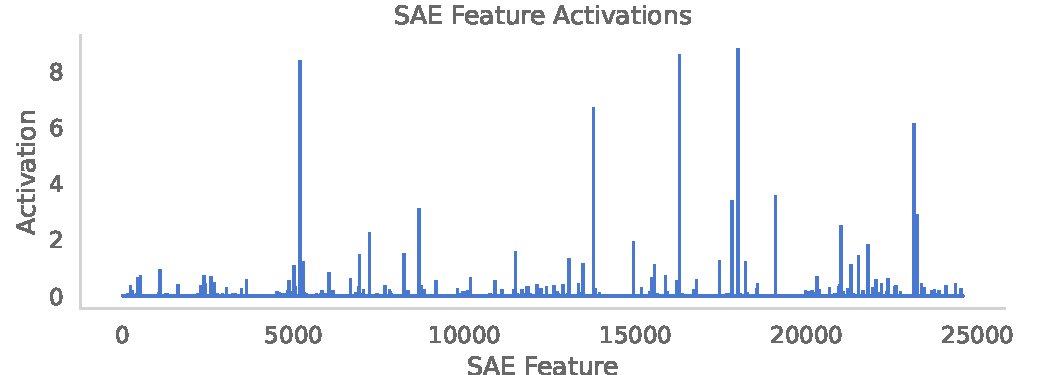
\includegraphics[width=\textwidth]{figures/sae_acts.pdf}
    \caption{
        The SAE feature activations for a sample prompt. Each line represents an activated feature, the bar along the bottom represents no activation.
        The lines are approximately double the thickness they would occupy for visual aid.
    }
    \label{fig:sae-acts}
\end{figure}

An SAE is an adaptor that takes a model layer's input and produces a replica of the layer's output.
In comparison to the model layer the SAE has a large hidden representation dimension in which sparsity is enforced (e.g. $24576$ for GPT-2 SAEs compared to $756$ \citep{saelens}).
This can be achieved in multiple ways such as clamping to the $k$ highest activations \citep{k-sparsity} or adding a sparsity regularising loss.
An example of an SAE activation is presented in \cref{fig:sae-acts} demonstrating the sparsity of the vector.
After training the elements of the SAE hidden dimension are given interpretations to better understand the model.
It is worth noting that SAEs have been shown to demonstrate subpar performance when used for interpretability \citep{saes-bad}.
In contrast, this thesis utilises SAEs to track model representation changes and spurious correlations, a use case \citet{saes-bad} suggest is still valid.

SAEs are challenging to train and so for the purposes of this project only pretrained SAEs are used.
\citet{saelens} provides a large collection of open source SAEs with their corresponding models.
This does limit the analysis as most models only have an SAE for a single layer.

\subsection{Metric Challenges}

As \citet{saes-bad} outline, SAEs do no provide a base truth for how the model represents concepts.
This means that using SAEs to extract concepts, or in the case of the project, using SAEs to evaluate the success of an adaptor will be imperfect.
Comparing across SAE features can give an insight into how a steering adaptor changes the models representation but not necessarily \emph{what} that new representation means as a human understandable concept.

The choice of metric is discussed in more detail in \cref{sec:steering-clear}.
Inherent challenges with SAEs are not addressed but rather the analysis takes into account their limitations.
